\documentclass{article}

\usepackage{amssymb}
\usepackage{soul}
\usepackage{float}
\usepackage{graphicx}
\usepackage{xcolor}
\usepackage{chngcntr}
\usepackage{mathrsfs}
\usepackage{centernot}
\usepackage[shortlabels]{enumitem}
\usepackage{verbatim}

\usepackage{geometry}  
\geometry{a4paper,left=10mm,right=10mm,top=2mm,bottom=2mm}
\usepackage{lastpage} %总页数
\usepackage{fancyhdr} 
\pagestyle{fancy}                   % 设置页眉页脚
\lhead{page \thepage\ of \pageref{LastPage}}   %页眉左侧显示页数                 
\chead{页眉中}                                  %页眉中
\rhead{\small\leftmark}                         %章节信息                       
\cfoot{\thepage}                                %当前页,记得调用前文提到的宏包                
\rfoot{页脚左}%                                                       
\lfoot{页脚右}
\renewcommand{\headrulewidth}{0.1mm} %页眉线宽,设为0可以去页眉线
\renewcommand{\footrulewidth}{0.1mm} %页脚线宽,设为0可以去页眉线



\usepackage[margin=1truein]{geometry}
\usepackage{setspace}
% Useful packages
\usepackage[colorlinks=true, allcolors=blue]{hyperref}
\usepackage{geometry}                		% See geometry.pdf to learn the layout options. There are lots.
\geometry{letterpaper}                   		% ... or a4paper or a5paper or ... 
%\geometry{landscape}                		% Activate for rotated page geometry
\usepackage[parfill]{parskip}    			% Activate to begin paragraphs with an empty line rather than an indent
\usepackage{graphicx}				% Use pdf, png, jpg, or eps§ with pdflatex; use eps in DVI mode
								% TeX will automatically convert eps --> pdf in pdflatex		
\usepackage{amssymb}
\usepackage{mathtools}
\usepackage{enumerate}
\usepackage{tikz}
\usepackage{fullpage,enumitem,amsmath,amssymb,graphicx,float,subfigure}
\usetikzlibrary{arrows}
\usepackage{listings}
\usepackage{tikz}
\usetikzlibrary{trees}
\usepackage{tikz-qtree}
\usepackage{xcolor}
% 定义可能使用到的颜色
\definecolor{CPPLight}  {HTML} {686868}
\definecolor{CPPSteel}  {HTML} {888888}
\definecolor{CPPDark}   {HTML} {262626}
\definecolor{CPPBlue}   {HTML} {4172A3}
\definecolor{CPPGreen}  {HTML} {487818}
\definecolor{CPPBrown}  {HTML} {A07040}
\definecolor{CPPRed}    {HTML} {AD4D3A}
\definecolor{CPPViolet} {HTML} {7040A0}
\definecolor{CPPGray}  {HTML} {B8B8B8}
\lstset{
    columns=fixed,       
    frame=none,                                          % 不显示背景边框
    backgroundcolor=\color[RGB]{245,245,245},            % 设定背景颜色
    keywordstyle=\color[RGB]{40,40,255},                 % 设定关键字颜色
    numberstyle=\footnotesize\color{darkgray},           % 设定行号格式
    commentstyle=\it\color[RGB]{0,96,96},                % 设置代码注释的格式
    stringstyle=\rmfamily\slshape\color[RGB]{128,0,0},   % 设置字符串格式
    breaklines,
    escapeinside=``,
    tabsize=3,
    extendedchars=false,
    showstringspaces=false,                              % 不显示字符串中的空格
    language=c++,                                        % 设置语言
    morekeywords={alignas,continute,friend,register,true,alignof,decltype,goto,
    reinterpret_cast,try,asm,defult,if,return,typedef,auto,delete,inline,short,
    typeid,bool,do,int,signed,typename,break,double,long,sizeof,union,case,
    dynamic_cast,mutable,static,unsigned,catch,else,namespace,static_assert,using,
    char,enum,new,static_cast,virtual,char16_t,char32_t,explict,noexcept,struct,
    void,export,nullptr,switch,volatile,class,extern,operator,template,wchar_t,
    const,false,private,this,while,constexpr,float,protected,thread_local,
    const_cast,for,public,throw,std},
}
\def\firstcircle{(90:1.75cm) circle (2.5cm)}
\def\secondcircle{(210:1.75cm) circle (2.5cm)}
\def\thirdcircle{(330:1.75cm) circle (2.5cm)}





\title{Stats 202 Final Project-QDH}
\author{David 06680631\\
        Kevin 06679923\\
        Yunjie Qu 06683920\\
        }

\begin{document}

\maketitle 

\tableofcontents
~\\
~\\
\section{Introduction}
\paragraph{} The Positive and Negative Syndrome Scale (PANSS), widely used in antipsychotic therapy, is a medical scale for the measurement of symptom severity of patients with schizophrenia. When assessing using PANSS, a patient was rated from 1 to 7 on 30 different symptoms based on reports and interviews. 
\paragraph{} The positive and negative scales, containing 7 items each, have a maximum score of 49 and a minimum score of 7, while the general psychopathology scale has 16 items and varies from 16 to 112. 

\paragraph{} In this report, we have four sample sets (A, B, C, and D) recording the details of every patient, as well as their PANSS and lead status. By these data, we first evaluated the effectiveness of the treatment, then lead status in E (a sample data missing the column LeadStatus) were predicted based on the four sample sets. Finally, a series of data science tools to achieve it were used, such as classification, clustering, and regression.

\section{Treatment effect}
\subsection{Introduction}
\paragraph{}In this section, we aim to find if treatment affects schizophrenia. We used the data sets A to D and create three new variables (the sum of positive : P Total), negative (N Total), and general (G Total), which add up to the scores of the three scales, respectively. 
 : \texttt{P\_Total}), negative (\texttt{N\_Total}), and general (\texttt{G\_Total}) which add up to the scores of the three scales, respectively.
\paragraph{}One challenge associated with treatment effect analysis was the initial status of patients in different groups. For example, the prior psychological status of a randomly selected patient from the treatment group may differ from that of a random patient in the control group. In these cases, even if significant differences in PANSS scores posterior to the treatment were implied, one would not be able to distinguish whether the" effect" came from the discrepancy in the prior distributions or the treatment, and the treatment effect was not well-identifies. 
	
		
	\paragraph{}The first step we did is to all the patients with no visiting day, i.e., VisitDay=0, showing 3000 samples. Of these 3000 patients, 1560 are in the control group while 1440 are in the treatment group. The reason for this selection is to ensure that the initial samples of the treatment group and the control group do not have significant differences. Otherwise, when the experiment's outcome shows a noticeable effect, we cannot conclude it is due to the treatment or the discrepancy of the prior distribution errors. To visualize this clearer, we draw them into histograms, distinguishing them based on the group. 


\begin{figure}[H]
\centering
\subfigure[\texttt{P\_Total}]{
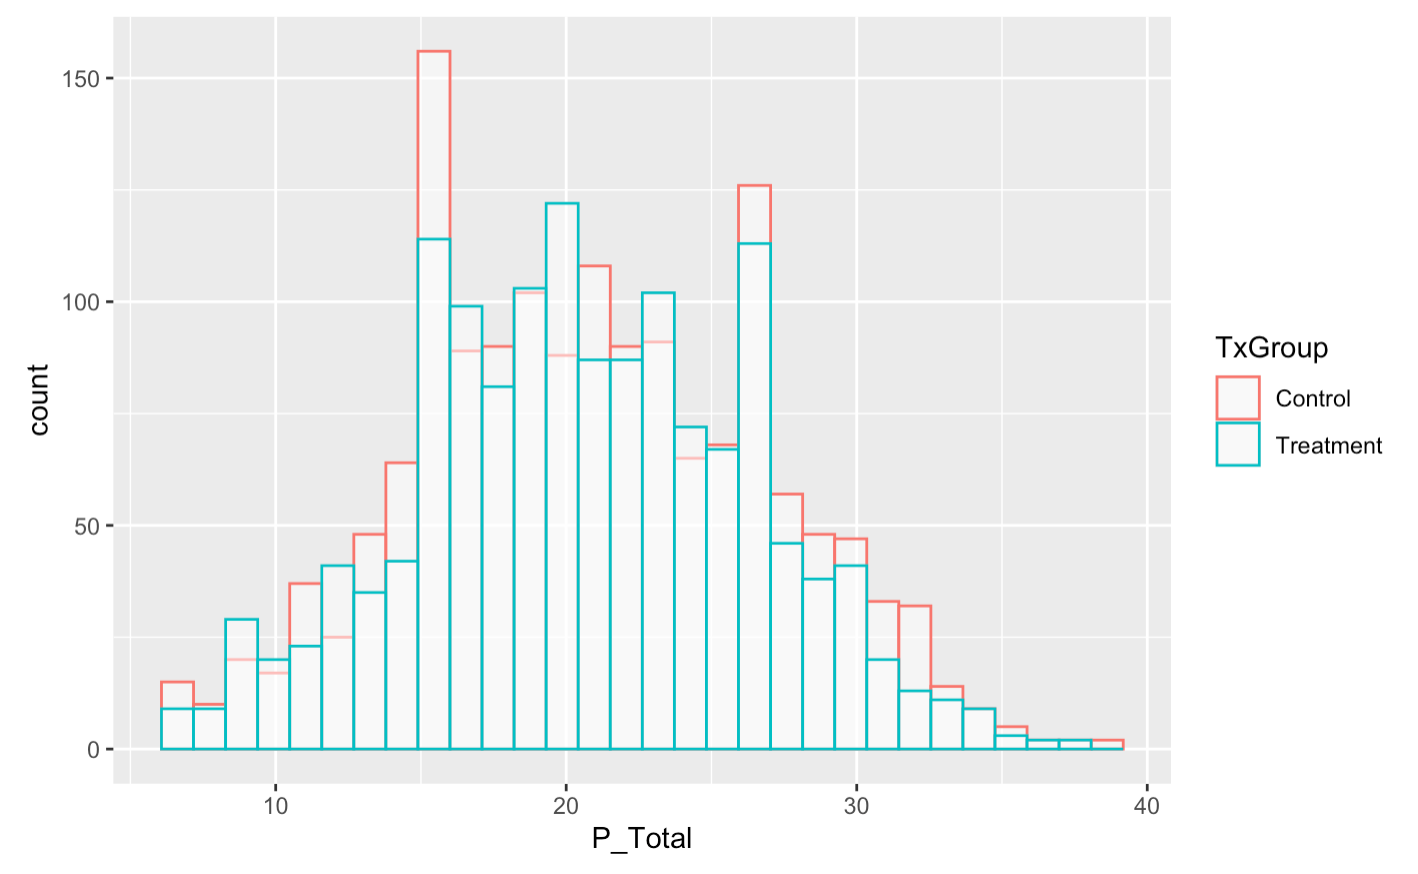
\includegraphics[width=7.7cm]{Q1.png}
%\caption{fig1}
}
\quad
\subfigure[\texttt{N\_Total}]{
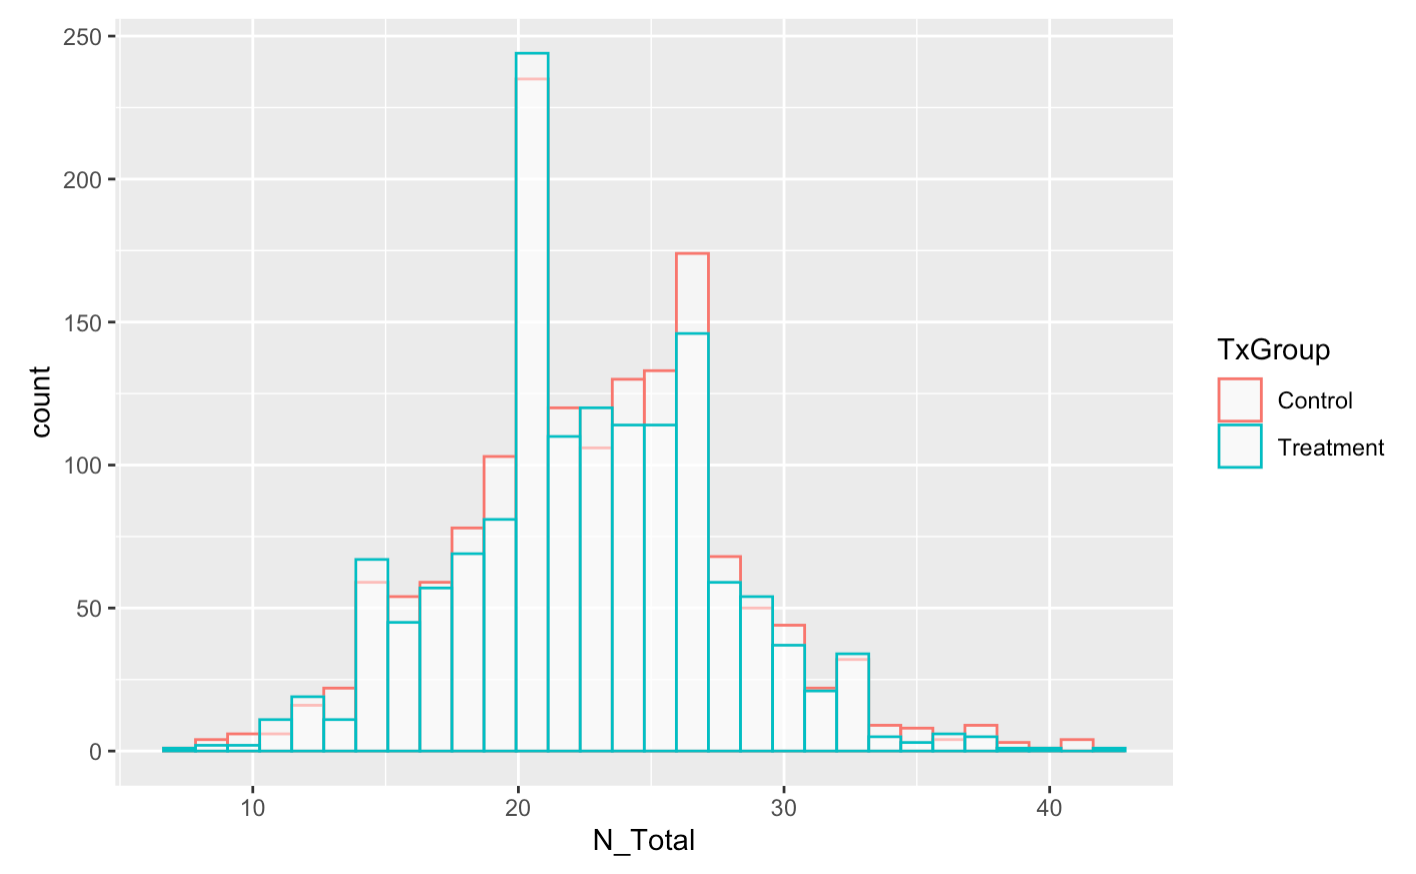
\includegraphics[width=7.7cm]{Q2.png}
}
\quad
\subfigure[\texttt{G\_Total}]{
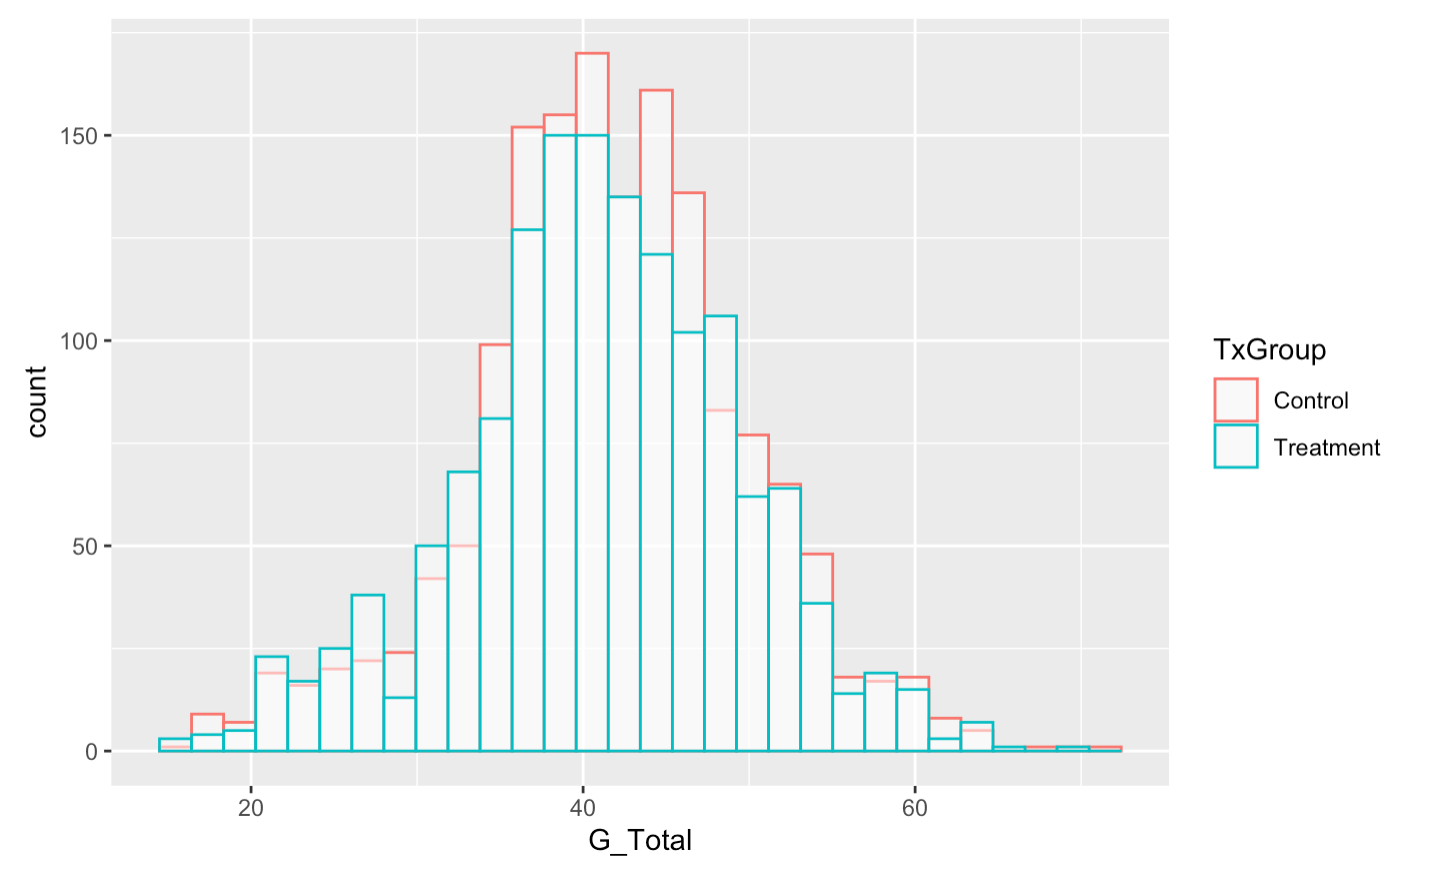
\includegraphics[width=7.7cm]{Q3.png}
}
\quad
\subfigure[\texttt{PANSS\_Total}]{
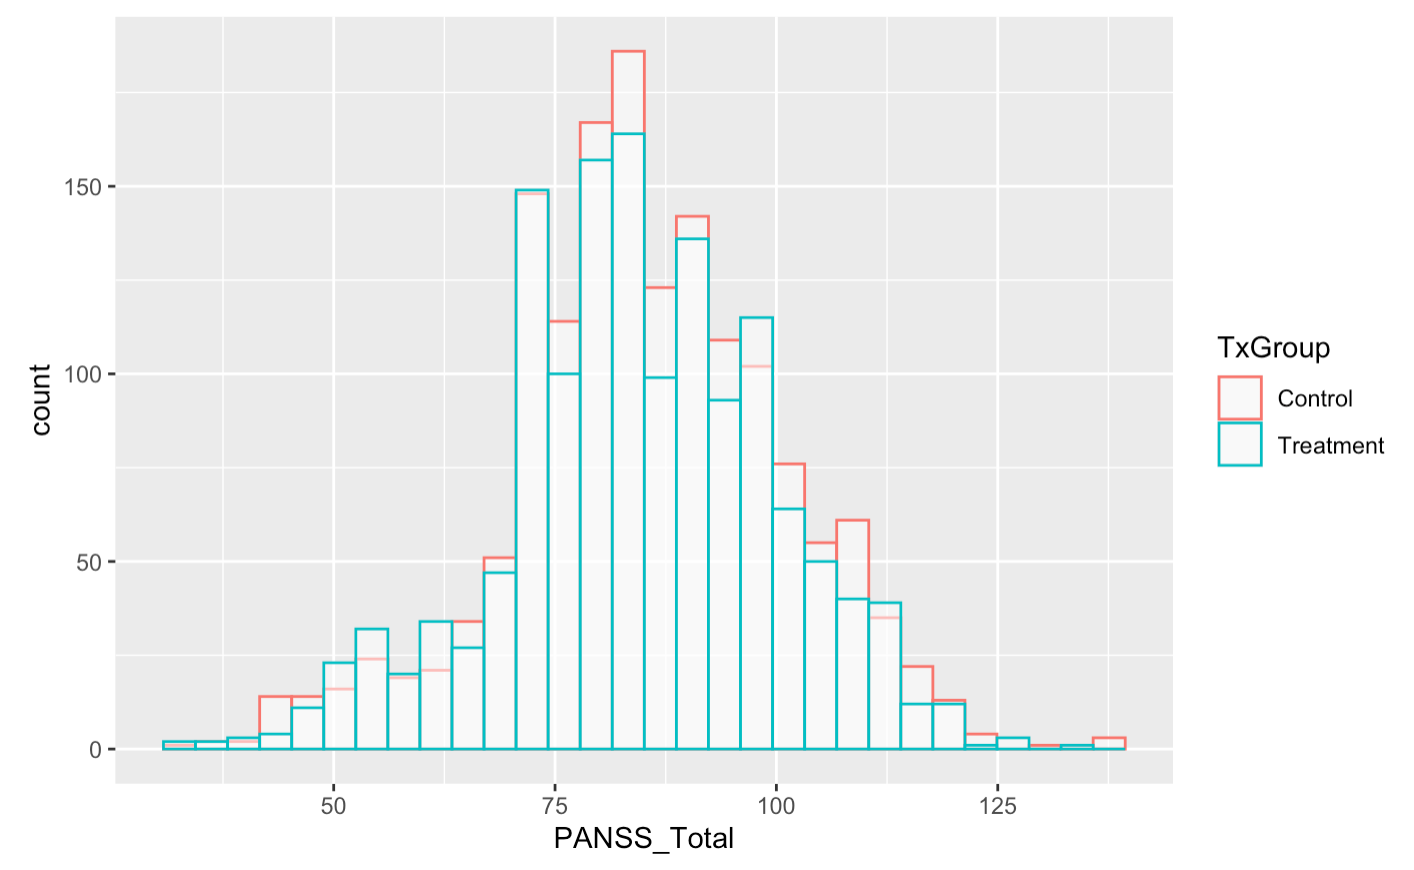
\includegraphics[width=7.7cm]{Q4.png}
}
\caption{ Histograms}
\end{figure}


\paragraph{}The next step is to check the distribution of visit days. Again, it revealed an apparent decreasing trend. Although it ranges from 0 to approximately 490, around one-third of it is the outlier which might deviate our analysis later. 
\begin{figure}[H]
		\centering
		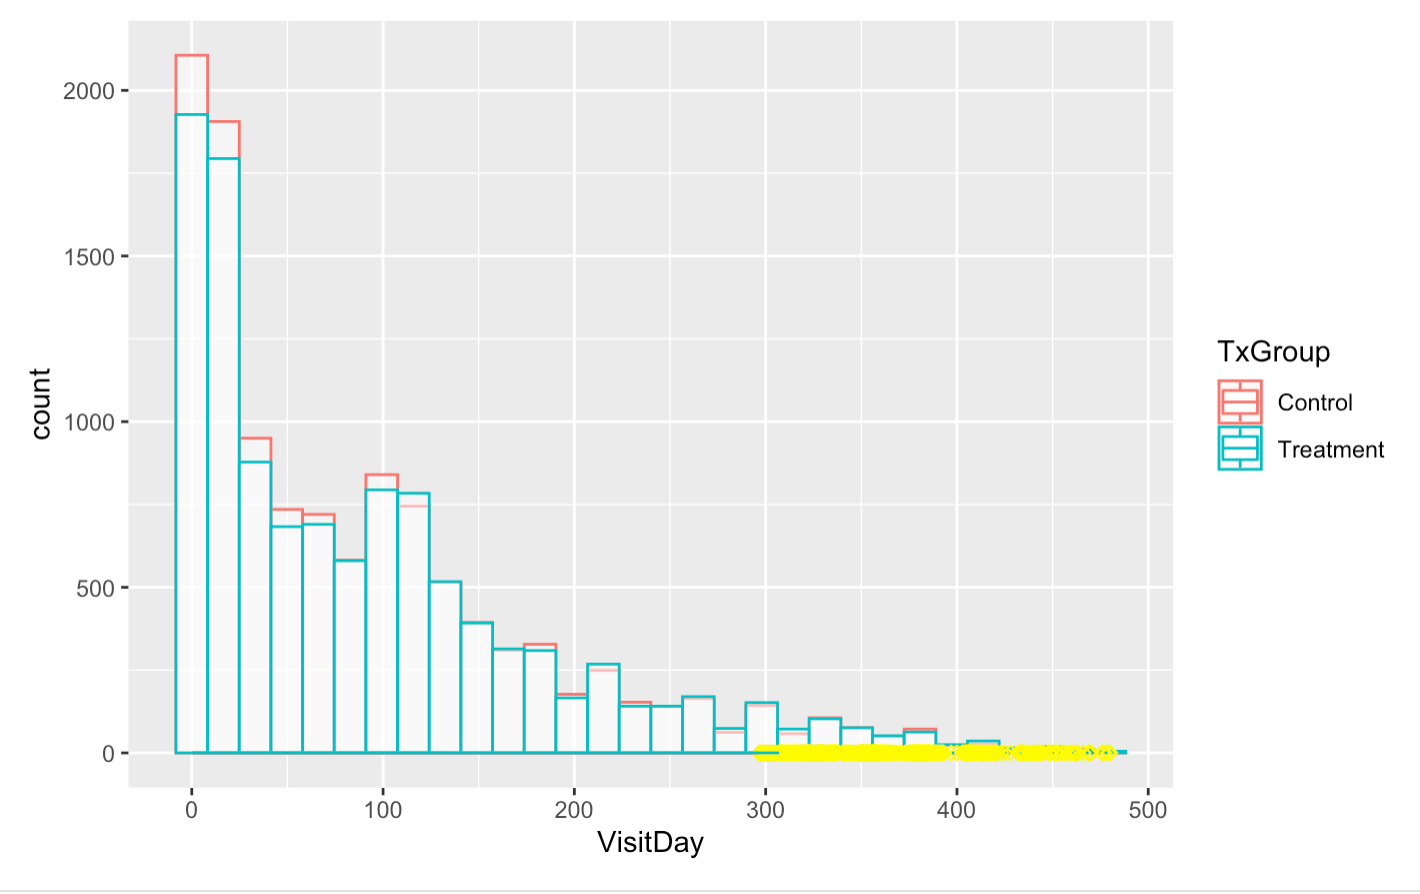
\includegraphics[width=9cm]{Q5}
		\caption{Distribution of visit days and outliers}
	\end{figure}	
	\paragraph{}There did not appear to be a noticeable difference between the treatment and control groups. Therefore, while it seems unlikely that a statistical test would suggest that the drug does have a significant effect on the patient, we proceeded with hypothesis testing to formally determine the effect of the drug. 
	
	\subsection{Visual inspection of treatment vs. control}
	\paragraph{}We first ploted `PANSS\_Total` vs `VisitDay`, for the `Treatment` and `Control` groups. 
	\begin{figure}[H]
		\centering
		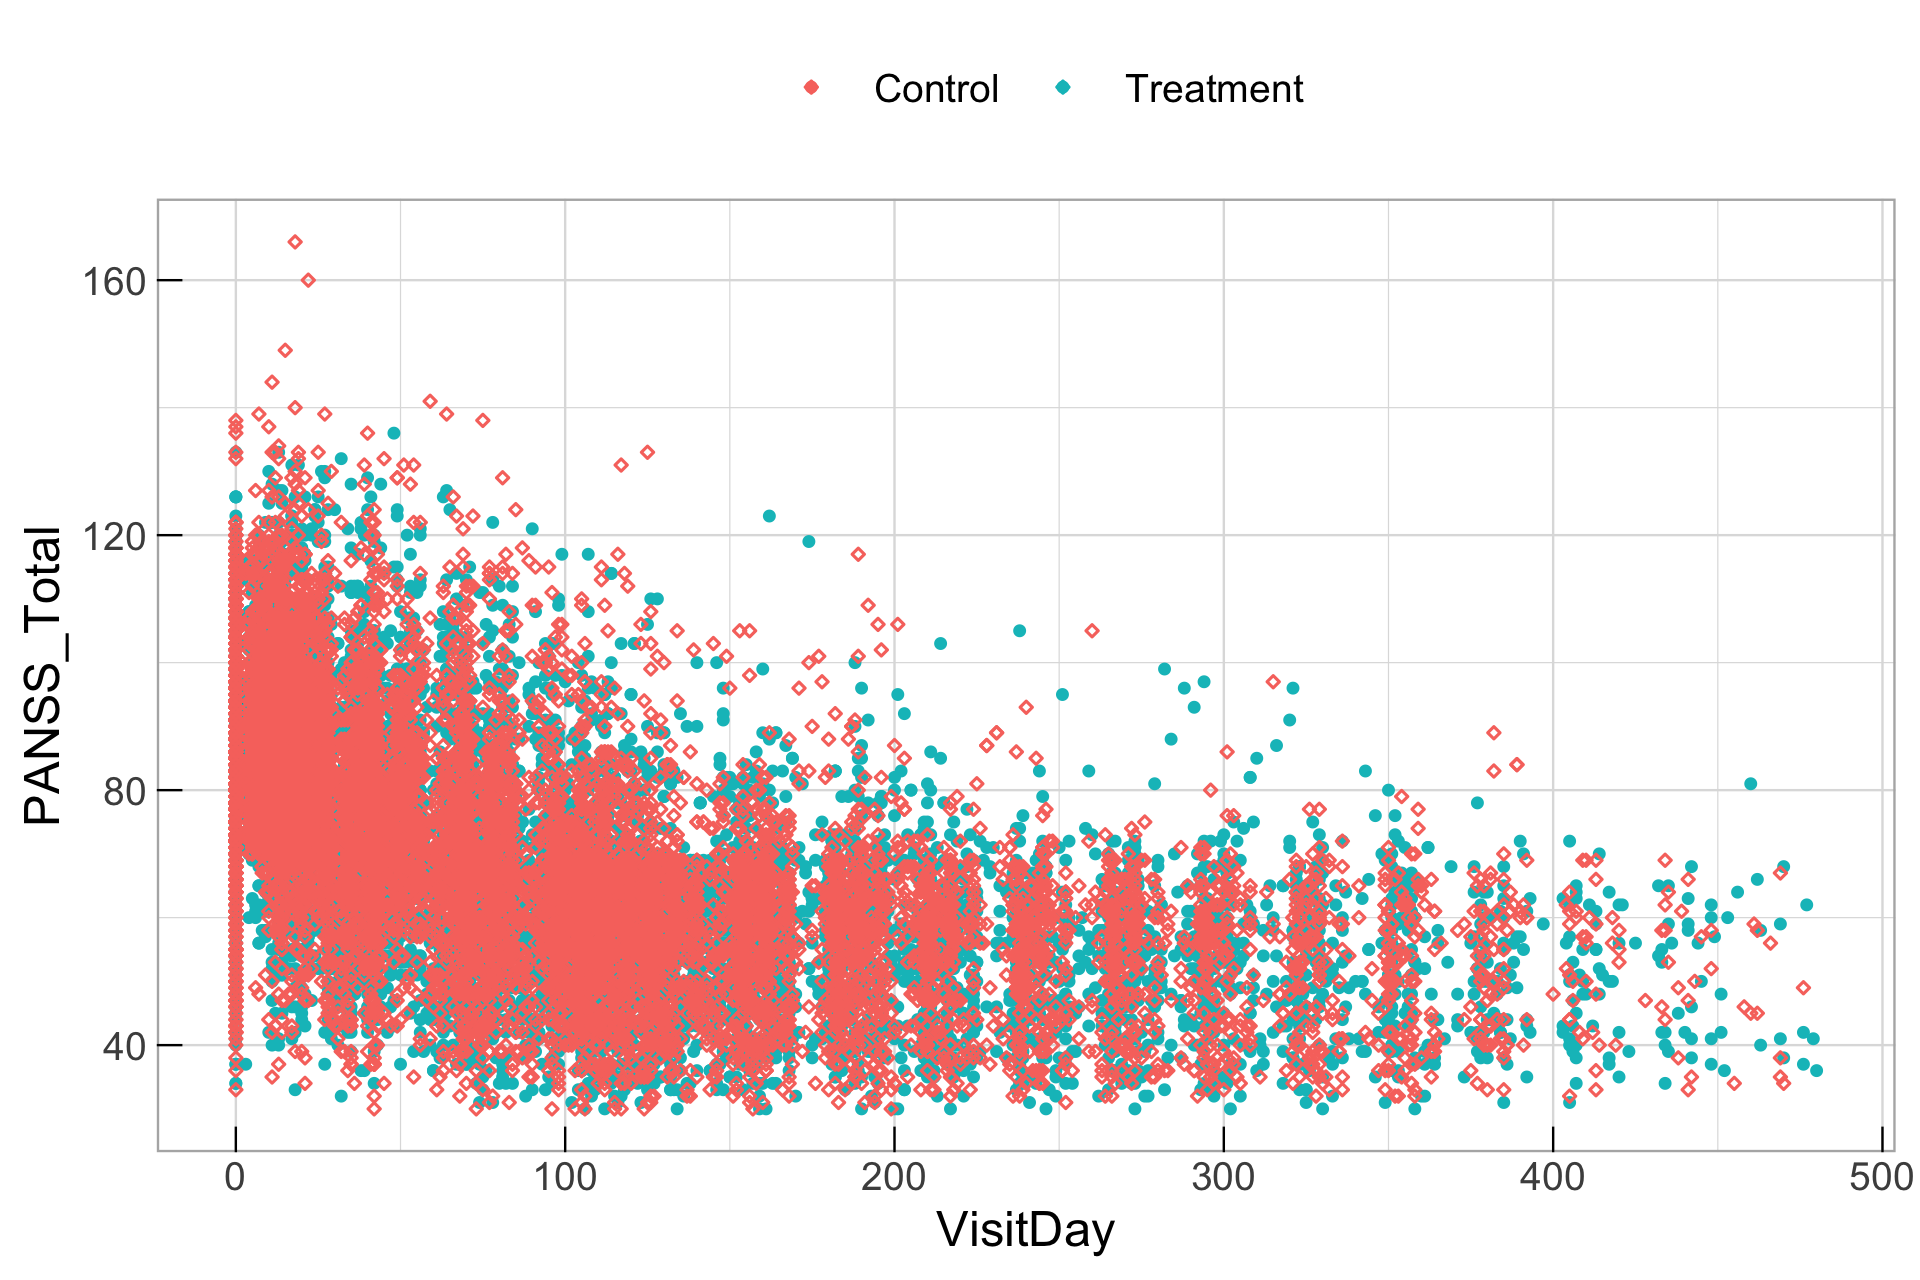
\includegraphics[width=1.0\linewidth]{pansstotal_vs_visitday.png}
		\caption{Scatter\_plot of \texttt{PANSS\_Total} Over Time }
	\end{figure}
\paragraph{}A plot of the total PANSS score over time did not seem to suggest a treatment effect. But to quantify this we did a linear regression on the total PANSS score vs time.
	\subsection{Identifying Treatment Effect with Primary Hypothesis}
	 Consider a regression of the total PANSS score on the patient’s visit day and an interaction term between visit day and the treatment group, where we set treatment group as 1 and control group as 0, i.e.:
	 \begin{equation}
	    PANSS_Total &= \beta_0 +\beta_1*VisitDay+\beta_2*VisitDay*Treatment 
	 \end{equation}  The null hypothesis is the treatment has no effect, i.e.: $\beta_2=0$. Performing equation 10 on R:
	 \begin{lstlisting}
## 
## Call:
## lm(formula = PANSS_Total ~ VisitDay + VisitDay:TxGroup, data = combined)
## 
## Residuals:
##     Min      1Q  Median      3Q     Max 
## -48.650  -9.686  -0.781   9.416  86.452 
## 
## Coefficients:
##                             Estimate Std. Error t value Pr(>|t|)    
## (Intercept)               81.6500051  0.1421343 574.457   <2e-16 ***
## VisitDay                  -0.1167884  0.0013669 -85.440   <2e-16 ***
## VisitDay:TxGroupTreatment -0.0007066  0.0015794  -0.447    0.655    
## ---
## Signif. codes:  0 '***' 0.001 '**' 0.01 '*' 0.05 '.' 0.1 ' ' 1
## 
## Residual standard error: 15.46 on 22906 degrees of freedom
## Multiple R-squared:  0.3317, Adjusted R-squared:  0.3317 
## F-statistic:  5685 on 2 and 22906 DF,  p-value: < 2.2e-16	 
	 \end{lstlisting}
The p-value of $\beta_0$ and $\beta_1$	are $\< 2e-16$ while $\beta_2=0.655$. Thus, we can confidently concluded that there is statistically no significant treatment effect under our given hypothesis, thereby confirming what we qualitatively observed in Figure 3.
	
\subsection{Other hypotheses}
\paragraph{}There are many alternatives to the specific hypotheses we considered. For example, we could take the same model form but regress the total score for a category (i.e., the sum of scores corresponding to negative symptoms only) and create a scatter plot of the total score for the category versus visit day to assess the effect of the treatment visually.
	\begin{figure}[H]
		\centering
		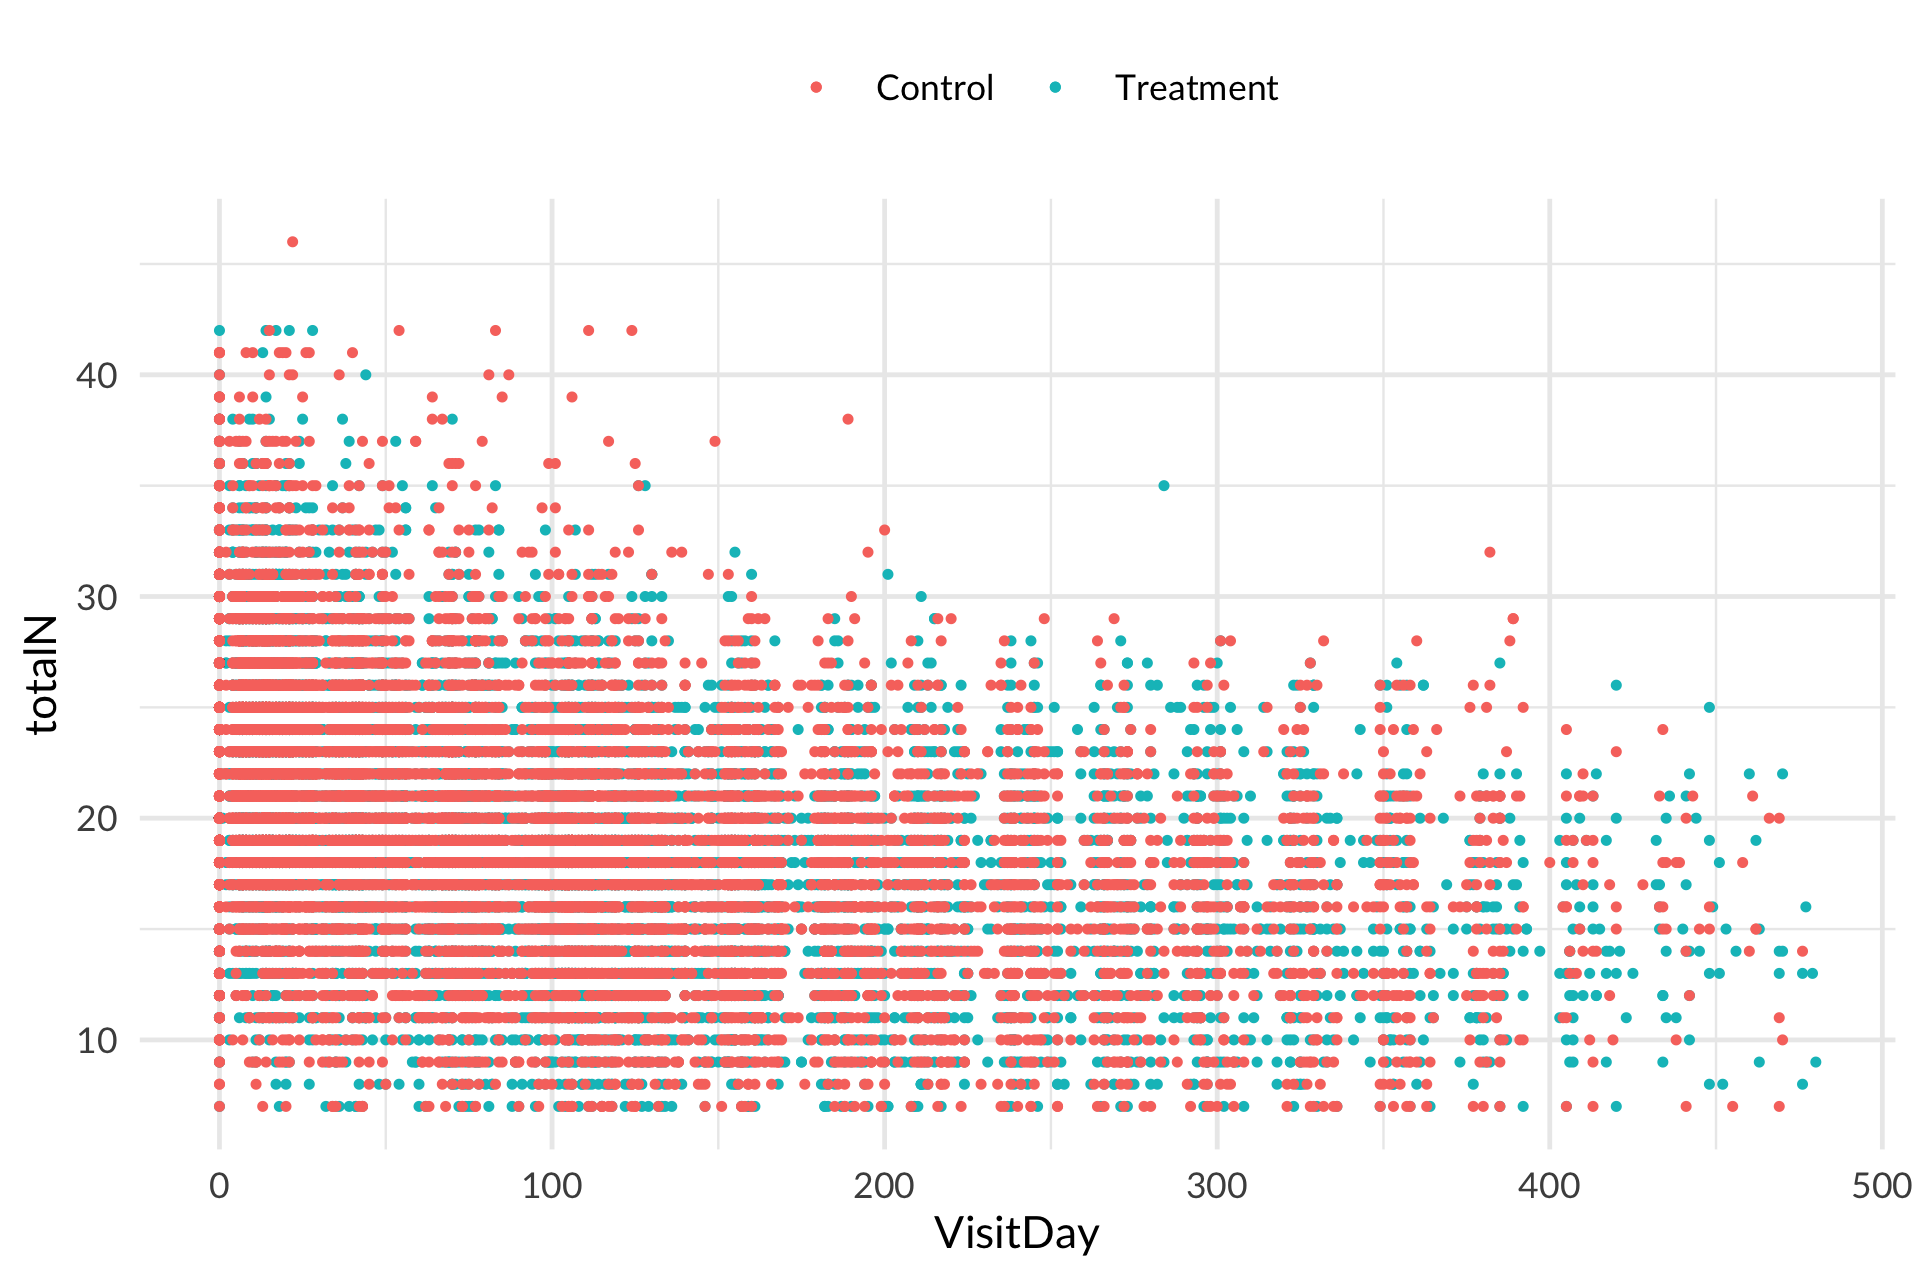
\includegraphics[width=0.8\linewidth]{panss_total_n.png}
		\caption{Scatter\_plot of \texttt{N\_Total} Over Time }
	\end{figure}
\paragraph{}The case of negative symptoms is shown in Figure 2. As before, we did not visualize a significant difference between the treatment and control groups.
Did the regression tests analogous to (1) but changing the response appropriately, We can safely conclude that there was no statistically significant effect of treatment on the full range of symptoms in a given category.


	\subsection{Summary} \paragraph{}Our conclusion: When it came to changes in their PANSS scores over time, there were no significant differences between the treatment and control groups. However, the scores themselves did decline over time; it was just that the driver of the decline did not seem to be the drug itself. What this tells us is that this means that either symptom decreased naturally over time, or perhaps the mere act of taking the scheduled assessment led to a decrease in symptoms. We believe that either hypothesis is intriguing and should be the focus of future research on schizophrenia.

\section{Patient segmentation}
	\subsection{Introduction}
	\paragraph{} For this task, we must use unsupervised learning to split the data into categories. 
Common methods used to cluster data are k-means and hierarchical clustering.
\paragraph{}We should not use hierarchical clustering in this case because:\\
1)	It does not scale well with large data sets.\\
2)	We are only interested in identifying patterns, not how similar individual observations are to other observations in the same cluster.\\
\paragraph{}Thus, we should go about using k-means clustering.
\begin{lstlisting}
Study.A <-read.csv(file.choose()) # Choose Study_A.csv
Study.B <-read.csv(file.choose()) # Choose Study_B.csv
Study.C <-read.csv(file.choose()) # Choose Study_C.csv
Study.D <-read.csv(file.choose()) # Choose Study_D.csv
Study.E <-read.csv(file.choose()) # Choose Study_E.csv
\end{lstlisting}

 \paragraph{}We will use Day 0 observations of datasets A-E and group them using k-means.
\begin{lstlisting}
Study.A <-subset(Study.A, VisitDay == 0)
Study.B <-subset(Study.B, VisitDay == 0)
Study.C <-subset(Study.C, VisitDay == 0)
Study.D <-subset(Study.D, VisitDay == 0)
Study.E <-subset(Study.E, VisitDay == 0)
\end{lstlisting}	
	\paragraph{}K-means can only be used on numeric values (in this case, the 30 features with values 1-7).
\paragraph{}All other features, such as study group, country, ID’s, lead status, etc., could be disregarded when clustering the data (we kept the study group temporarily for the initial observations).
\paragraph{}We could also disregard the PANSS total because it yielded no new information if we already have the individual PANSS values.
\begin{lstlisting}
Study.A <- Study.A[, -which(names(Study.A) %in% c("Country", "PatientID", "SiteID", "RaterID", "AssessmentID", "TxGroup", "VisitDay", "PANSS_Total", "LeadStatus"))]
Study.B <- Study.B[, -which(names(Study.B) %in% c("Country", "PatientID", "SiteID", "RaterID", "AssessmentID", "TxGroup", "VisitDay", "PANSS_Total", "LeadStatus"))]
Study.C <- Study.C[, -which(names(Study.C) %in% c("Country", "PatientID", "SiteID", "RaterID", "AssessmentID", "TxGroup", "VisitDay", "PANSS_Total", "LeadStatus"))]
Study.D <- Study.D[, -which(names(Study.D) %in% c("Country", "PatientID", "SiteID", "RaterID", "AssessmentID", "TxGroup", "VisitDay", "PANSS_Total", "LeadStatus"))]
Study.E <- Study.E[, -which(names(Study.E) %in% c("Country", "PatientID", "SiteID", "RaterID", "AssessmentID", "TxGroup", "VisitDay", "PANSS_Total", "LeadStatus"))]
\end{lstlisting}

\paragraph{}Combine into one dataset.
\begin{lstlisting}
Combined.Studies <- rbind(Study.A, Study.B, Study.C, Study.D, Study.E)
\end{lstlisting}
	\subsection{Initial Observations}
	\paragraph{} Before determining the optimal k value for k-means clustering and implementing it, let us first view the trends in each study group when viewing the data along two principal components with the fviz and prcomp functions.

\begin{lstlisting}
library(factoextra)
fviz(prcomp(Combined.Studies[, -1]), "ind", label = "none", habillage = Combined.Studies$Study, addEllipses = "True", alpha=0.5)
\end{lstlisting}
	
	\begin{figure}[H]
		\centering
		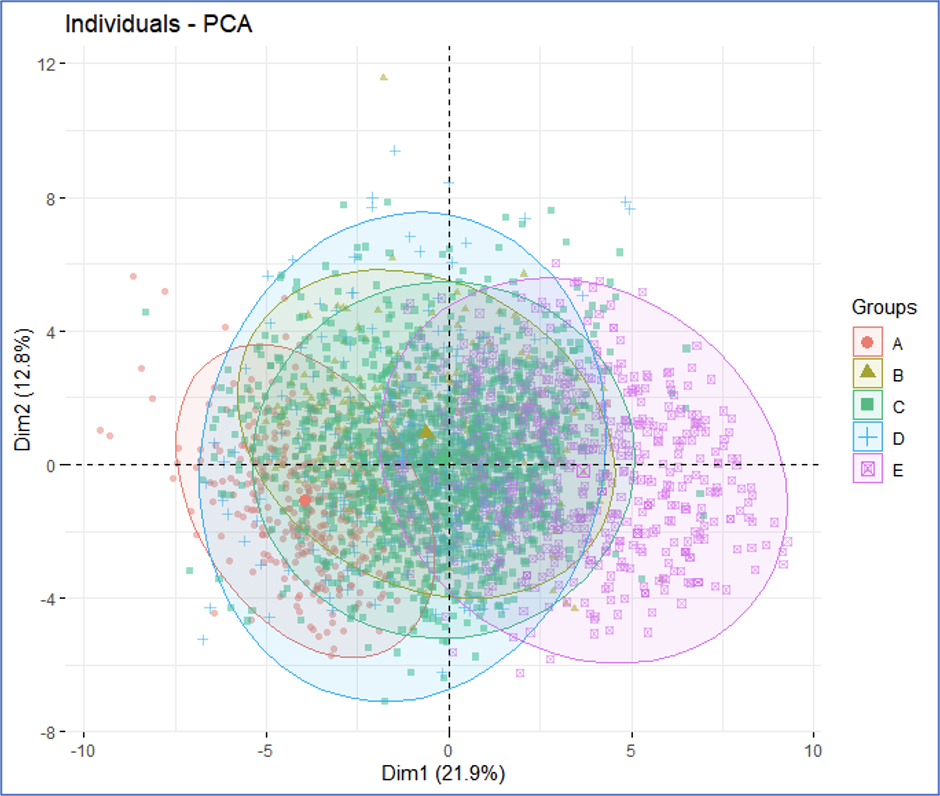
\includegraphics[width=15cm]{Q21.png}
		\caption{PCA}
	\end{figure}
	\paragraph{}This provides a rough visualization of the clusters of observations based on the study. It can be seen that while Studies A-D was relatively close to each other, Study E noticeably had a much higher average first principal component value. On the other hand, study A also had a lower average first principal component value. This was covered later with further analysis of the principal component values.


	\subsection{K-Means Clustering}
	\paragraph{} Now that we have chosen k-means as the preferred method, we must know how many clusters to choose. This can be done with the help of the factoextra library. Specifically, we can use the fviz_nbclust method to gather more information on choosing the optimal value of k for the k-means clustering method. We can also get rid of the study values now.
	
	\begin{lstlisting}
Study.A <- Study.A[, -which(names(Study.A) %in% c("Study"))]
Study.B <- Study.B[, -which(names(Study.B) %in% c("Study"))]
Study.C <- Study.C[, -which(names(Study.C) %in% c("Study"))]
Study.D <- Study.D[, -which(names(Study.D) %in% c("Study"))]
Study.E <- Study.E[, -which(names(Study.E) %in% c("Study"))]
Combined.Studies <- Combined.Studies[, -which(names(Combined.Studies) %in% c("Study"))]
	\end{lstlisting}
	
	\paragraph{}K-means is sensitive to outliers and noisy data if not standardized, and standardizing the data accounts for the different variances of each feature. Therefore, instead of measuring the raw value, the data should be measured by the number of standard deviations from the mean.
	\begin{lstlisting}
Study.A <- scale(Study.A)
Study.B <- scale(Study.B)
Study.C <- scale(Study.C)
Study.D <- scale(Study.D)
Study.E <- scale(Study.E)
Combined.Studies <- scale(Combined.Studies)
	\end{lstlisting}
\paragraph{}	\textbf{Average Silhouette Method}– measures how well each observation is contained within its cluster. A higher average silhouette width generally means a good clustering. In this case, the appropriate number of clusters to choose is 2.
\begin{lstlisting}
fviz_nbclust(Combined.Studies, kmeans, method = "silhouette") + labs(subtitle = "Silhouette method")
\end{lstlisting}	
	
\paragraph{}	\textbf{Elbow Method} – defines clusters by minimizing the within sum of squares error (WSS) as a function of the number of clusters. WSS measures how close together a cluster is, and generally a smaller WSS is better. As for selecting an appropriate number of clusters, locations of a bend (in this case at 2 clusters) is considered an appropriate number.
\begin{lstlisting}
fviz_nbclust(Combined.Studies, kmeans, method = "wss") + geom_vline(xintercept = 2, linetype = 2) + labs(subtitle = "Elbow method")
\end{lstlisting}	

\paragraph{}	\textbf{Gap Statistic Method}– measures the within intra-cluster variation as a function of the number of clusters chosen. For this method, the ideal number of clusters is the smallest value of k such that its gap statistic is within one standard deviation of the value that maximizes the gap statistic. The ideal number here is 9 since it is the greatest value smaller than 10 that is within 1 standard deviation. However, we can see that at 2 clusters, the gap value is comparable to the gap value at 3 clusters since the difference is somewhat negligible.
\begin{lstlisting}
 fviz_nbclust(Combined.Studies, kmeans, nstart = 25,  method = "gap_stat", nboot = 100) + labs(subtitle = "Gap statistic method")
\end{lstlisting}

\begin{figure}[htbp]
\centering

\subfigure[Average Silhouette Method]{
\begin{minipage}[t]{0.3333333\linewidth}
\centering
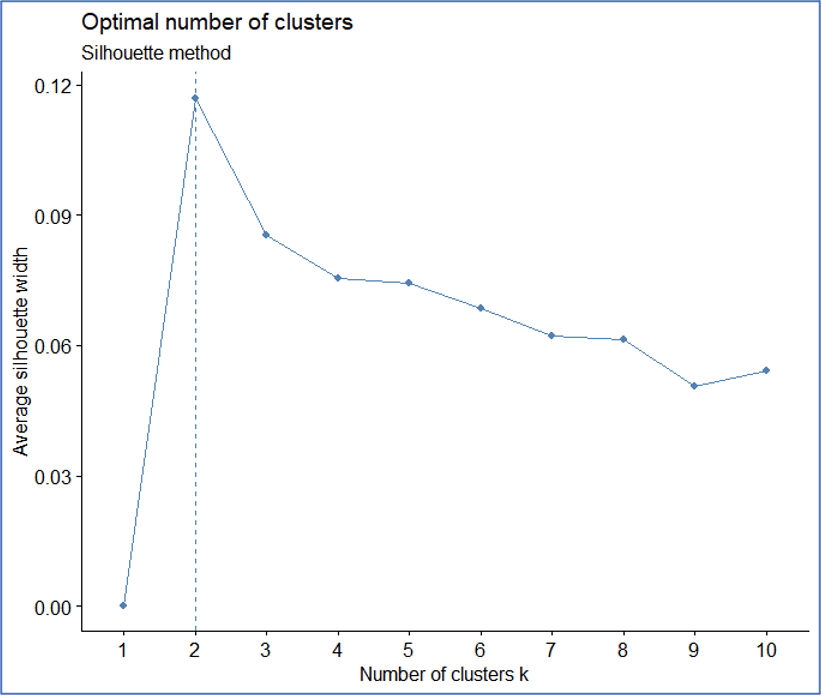
\includegraphics[width=2.21in]{Q22.png}
%\caption{fig1}
\end{minipage}%
}%
\subfigure[Elbow Method]{
\begin{minipage}[t]{0.3333333\linewidth}
\centering
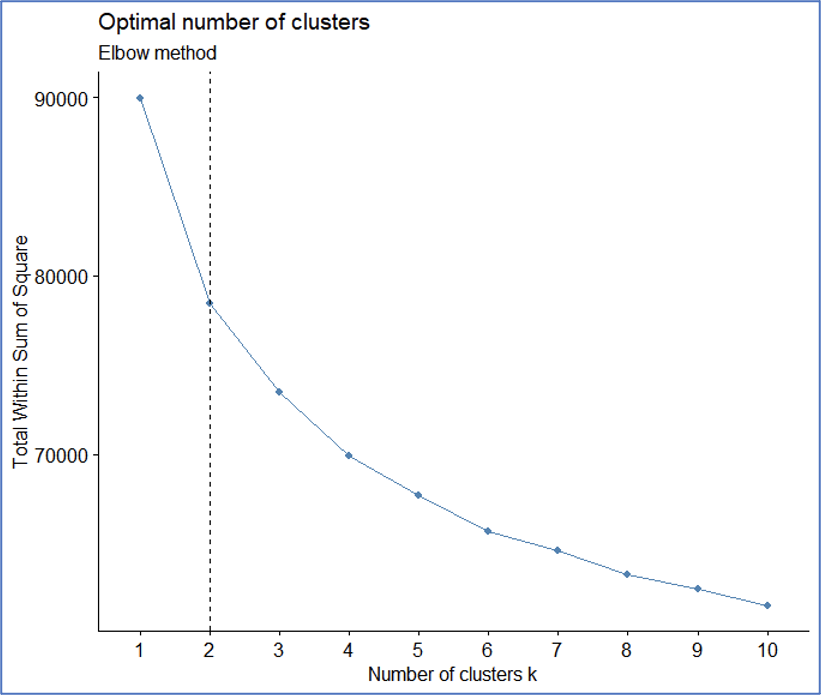
\includegraphics[width=2.21in]{Q23.png}
%\caption{fig2}
\end{minipage}%
}%
                 %这个回车键很重要 \quad也可以
\subfigure[Gap Statistic Method]{
\begin{minipage}[t]{0.3333333\linewidth}
\centering
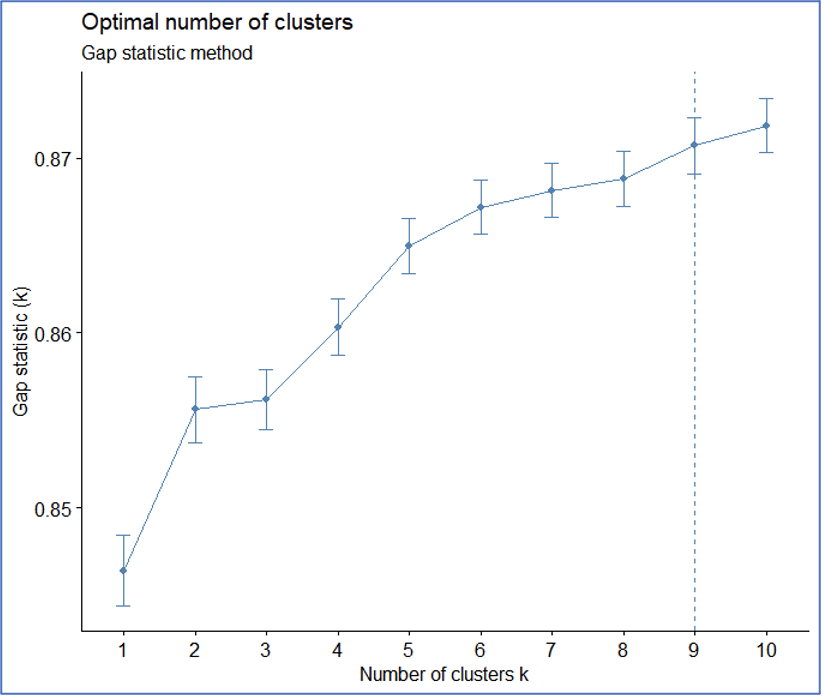
\includegraphics[width=2.21in]{Q24.png}
%\caption{fig2}
\end{minipage}
}%

\centering
\caption{3 Methods}
\end{figure}
	
\paragraph{}	\textbf{NbClust()} – The final way we can determine the optimal number of clusters is by using this function from the NbClust library. It provides 30 indices for determining the appropriate number of clusters and determines the number of clusters using a majority vote. More information about the 30 indices can be found in the NbClust library documentation.

\begin{lstlisting}
library(NbClust)
NbClust(data = Combined.Studies, distance = "euclidean", min.nc = 2, max.nc = 10, method = "kmeans")
\end{lstlisting}

\begin{lstlisting}
******************************************************************* 
* Among all indices:                                                
* 11 proposed 2 as the best number of clusters 
* 4 proposed 3 as the best number of clusters 
* 5 proposed 4 as the best number of clusters 
* 1 proposed 5 as the best number of clusters 
* 1 proposed 6 as the best number of clusters 
* 1 proposed 10 as the best number of clusters 
                   ***** Conclusion *****                            
* According to the majority rule, the best number of clusters is 2
*******************************************************************
\end{lstlisting}
\paragraph{}Now that we choose k = 2, we can partition the dataset using 2-means clustering.
\begin{lstlisting}
kmeans.clust <- kmeans(Combined.Studies, 2, nstart = 100)
fviz_cluster(kmeans.clust, Combined.Studies, geom = c("point")) + labs(title = "2-Means Clustering")
\end{lstlisting}
\begin{figure}[H]
		\centering
		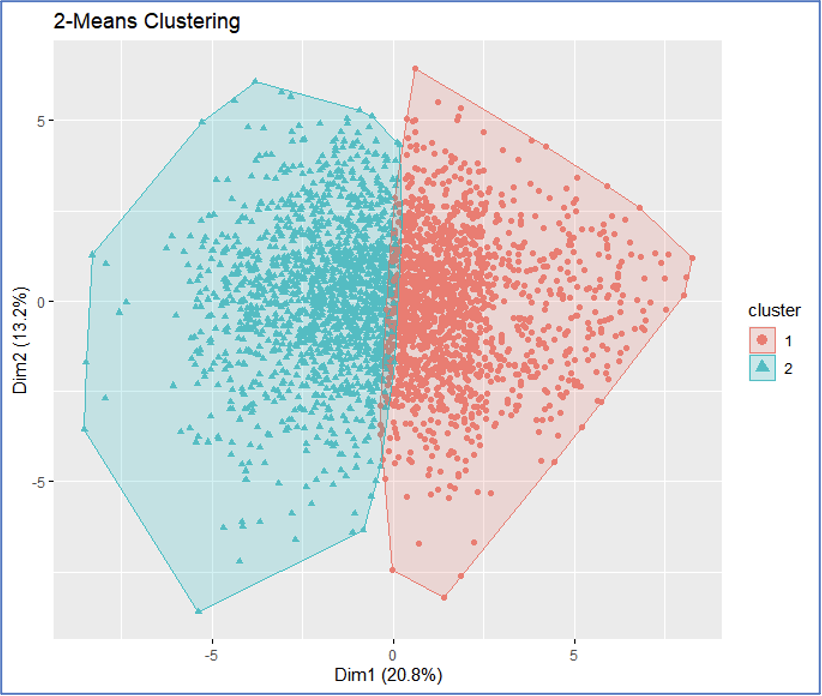
\includegraphics[width=11cm]{Q25.png}
		\caption{2-Means Clustering}
	\end{figure}
	\paragraph{}Only two dimensions are shown here from a reduction of 30 dimensions because the k-means clustering algorithm shows the data in a system of two principal components. Clusters 1 and 2 can be separated relatively well along the first principal component switches from positive to negative (where Dim1 ≈ 0).

	\subsection{Analysis}
	\paragraph{} The k-means clustering with k = 2 shows that the data forms two distinct groups when visualized using two principal components. However, we did not yet know what these two principal components mean in terms of the original features of the data. This might be useful since we can conclude the reasoning behind how these two groups were formed.
\paragraph{} For example, because we knew that the two clusters are separated along the first principal component (where Dim1 ≈ 0), if we knew which features contributed most to a change in the first principal component, we could figure out how exactly these two groups of patients are split.
\paragraph{}To dig further on this matter, a principal component analysis using the built-in R function prcomp() can be used again to determine each feature's contributions to each principal component.

\begin{lstlisting}
results <- prcomp(Combined.Studies)
results$rotation <- -1 * results$rotation #Eigenvectors in R by default point in the negative direction. This reverses the signs.
results$x <- -1 * results$x #This reverses the signs of the principal component scores for each observation as well.
biplot(results, scale = 0) #This is a little cluttered, we can visualize the graph without the observation points.
\end{lstlisting}	
	\begin{figure}[H]
		\centering
		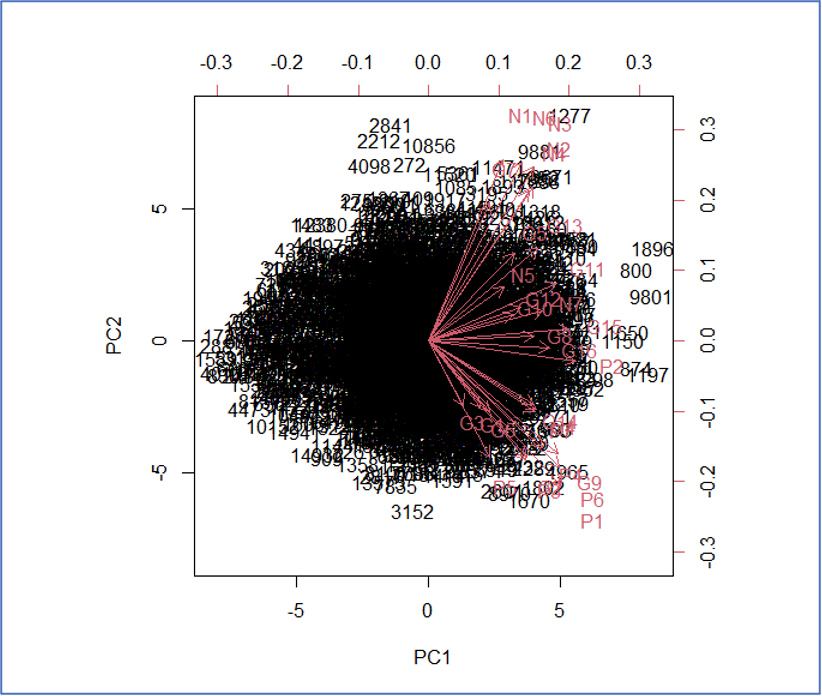
\includegraphics[width=11cm]{Q26.png}
		\caption{ The contributions each feature makes to each principal component (using the prcomp() method)}
	\end{figure}

\begin{lstlisting}
biplot(results, col = c("white", "red"), scale = 0)
\end{lstlisting}

	\begin{figure}[H]
		\centering
		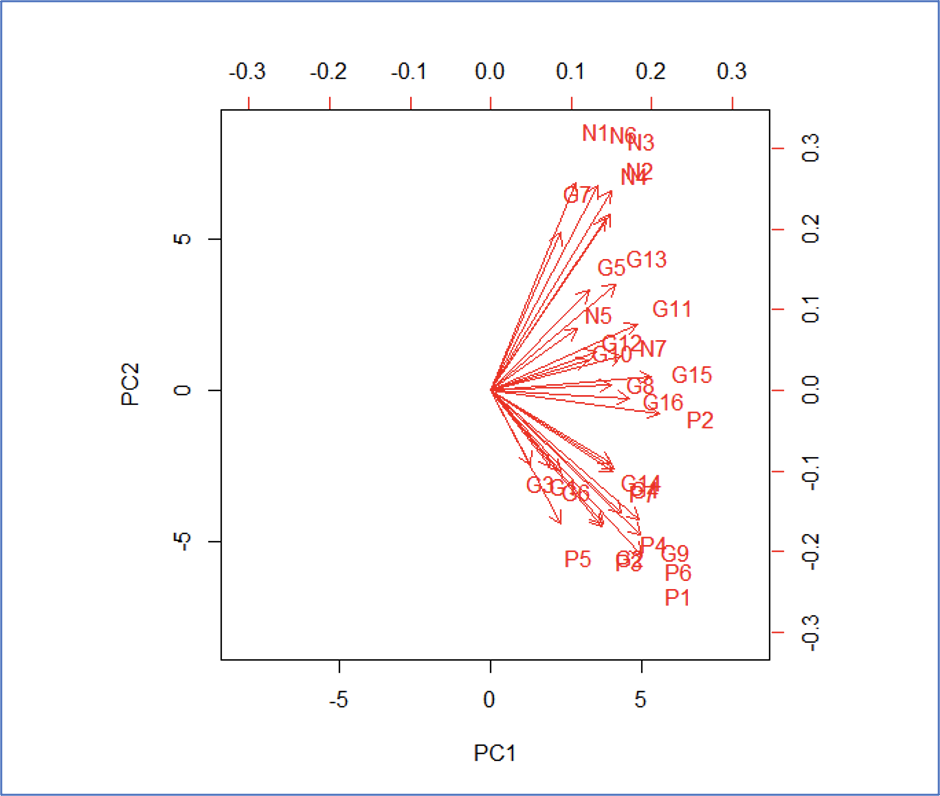
\includegraphics[width=11cm]{Q27.png}
		\caption{biplot}
	\end{figure}
\paragraph{} From this, we can see the proportion that each feature contributes to the two principal components. Since we are mostly interested in the first principal value since the clusters are split near when its value 0, we can see that the features that contribute most to PC1 (vectors furthest right on the graph) are P2, G15, P1, P6, G9, G11, P4, G4, P7, etc. This shows that the clusters are mainly divided on how patients scored on the positive and general symptoms. Indeed, a quick look at the trends in each cluster show that the left cluster (cluster 2) has mostly patients who scored higher on these symptoms while the right cluster (cluster 1) has mostly patients who scored lower on these symptoms.

\begin{lstlisting}
kmeans.clust$centers
\end{lstlisting}

\begin{lstlisting}

    P1         P2         P3         P4         P5         P6
1  -0.4724259 -0.5346738 -0.3816866 -0.4048736 -0.2373839 -0.4758130
2 	 0.5083891  0.5753756  0.4107423  0.4356944  0.2554547  0.5120341

    P7         N1         N2         N3         N4         N5
1 	 -0.3946165 -0.2128975 -0.3249632 -0.2962271 -0.3168242 -0.2546761
2 	  0.4246565  0.2291042  0.3497008  0.3187773  0.3409423  0.2740633

    N6         N7         G1         G2         G3
1  -0.2698701 -0.3386144 -0.1385484 -0.3177588 -0.09534452
2 	 0.2904139  0.3643912  0.1490953  0.3419481  0.10260258

    G4         G5         G6         G7         G8         G9
1  -0.3395045 -0.2556141 -0.1872483 -0.1533706 -0.3787357 -0.4751995
2 	 0.3653491  0.2750726  0.2015025  0.1650459  0.4075667  0.5113738
 
    G10         G11         G12         G13         G14         G15
1  -0.2861119 -0.3900442 -0.3216501 -0.3415269 -0.3713398 -0.4730922
2 	 0.3078921   0.4197361  0.3461356  0.3675255  0.3996078  0.5091062

    G16
1  -0.4152765
2 	 0.4468892
\end{lstlisting}

\paragraph{}As for the initial observations from earlier, we can now explain them using this new information. From the principal component analysis, we can see that points with a higher first principal component value tend to score poorly on the positive and general symptoms. Since much of Study E lies in cluster 1, we can conclude that the study differs from the other studies due to patients scoring lower in these positive and general symptoms on average. The opposite can be said for Study A, where the patients score higher on these symptoms on average.


\section{Forecasting}
	\subsection{Thought Process} 
	\paragraph{} The goal is to predict the total PANSS score (across the 30 PANSS symptoms) for the 18th-week assessment.After discussion, we felt that we should not simply define $week 18$ as a visit when $visitDay=126$, due to differences in when patients participated in the study and when they withdrew from the study. Therefore, we felt that $week 18$ should be defined as the week after the patient's last recorded visit date. This is, of course, a rather imprecise approximation, but we think it makes more sense than simply defining it as visitDay=126. 
	\paragraph{} We used country, treatment group, visit day, and study group as predictors for prediction. The SiteID was omitted because we did not know where they would be evaluated. The RaterID was not considered a predictor because we did not know who would evaluate them. When it comes time to predict, we specify a patient ID which then sets the above-listed predictors except for VisitDay. In our prediction, the test set is the "18th week" for the 513 patients in study E.
	\subsection{Data processing}
	 \textbf{Step1}. Load the csvs and choose the columns corresponding to the prediction and combine. \\
	\textbf{Step2}. Find the final visit day for each patient and creat the test set by choosing the patients whose VisitDay==FinalDay.Remove the patients who were assessed multiple times in the same day by the same person and at the same location (for example, PatientID 50505) and average the 'PANSS\_Total'.\\
	\textbf{Step3}. Add a value of 7 days to their `VisitDay` and create "'naive\_forecast.csv" submission\\
	\textbf{Step4}. To remove some variance from naive prediction, we take the simple average of these last two visit scores. First, we need to take note of the `VisitDay` and `PANSS\_Total` for the second to last day. Average final two scores and creat submission "less-naive-forecast.csv". \\
	\textbf{Step5}. Repeat this process, storing data for the third and fourth day.\\
	\textbf{Step6}. Exponential smoothing.	\\
    \textbf{Step7}. Create training set: remove test from total, remove any duplicates as we did for the test set and average over cases where all is identical except for the total PANSS score.\\
    Step8. Do the other methods: Gradient boosting,random Forest,linear regression,lasso regression,ridge regression
	,Naive Forecast.
	\paragraph{} We created a baseline prediction by considering the most naive prediction method possible. In this case, the most naive approach was to use each patient's most recent PANSS total score as the score we would expect them to have at their week 18 visit (i.e., their next visit). While the idea behind this approach was relatively crude, this score alone would put our team at #3 on the leaderboard at the time of this writing. The reason might be that the PANSS total score no longer changes as a function of VisitDay for a long time. Because the total score did not change significantly at the end of the study, it was an excellent way to use the most recent score to predict future values. To remove some variance from naive prediction, we thought to take the simple average of the last two visit scores, but the way performed relatively poorly on the test set (the public leaderboard on Kaggle has a poor rank). To weigh historical data that did not follow a strong trend (i.e., patient scores near the end of the study), we thought of other methods.
\subsection{Other methods}
 \textbf{xgboost (Gradient boosting)},
      \textbf{random Forest},
    \textbf{linear regression},
    \textbf{lasso regression},
    \textbf{ridge regression} are all shown in "Gradient Boosting(h2o).Rmd".
  \paragraph{}These methods were not discussed here because they produce test results that rank very low on Kaggle. For example, the random forest model produces test results with a value of 11.38179 on the public Kaggle ranking, which would almost rank last. We attributed this poor performance to the inherent difficulties of tree-based methods in prediction. Tree-based methods could not predict values outside the range observed in the test set (since the node value was calculated as the average of the included observations). When we examined the scores predicted by these models at week 18, the range of values was much smaller than those at week 17 for the patients in Study E.
  

	\subsection{Exponential smoothing}
	\paragraph{}By comparison, we found that the most productive approach is to optimize the naive forecasting method. The most obvious way is to incorporate more historical data into the week 18's forecasts. In time series analysis, this is known as "exponential smoothing". In exponential smoothing, we treated each observation as a linear combination of the two previous observations:
	\begin{equation}
	  y_i = \alpha y_{i-1}+(1-\alpha)y_{i-2}  
	\end{equation}
where in this problem $y_i$ denote the $ith$ total PANSS score and $ 0<\alpha<1$ is the smoothing factor.This equation defined a recursive relationship that went back to the initial set of observations related to time. In this equation, we saw that α determines the relative importance given to historical data (when $\alpha$ approaching 1, the equation represent the naive prediction in (4.2).
Therefore, to improve the performance exhibited by the naive predictions, we used exponential smoothing for a range of values of α to truncate the recurrence relationship at the appropriate number of terms (so that the truncation error is less than $0.5 \%$). Specifically, we considered values of $\alpha$ = 0.9, 0.8, and 0.7, and we considered only the two, three, and four most recent time points for truncation, respectively. At the time of writing, these lowest scores placed our team at the top two of the public rankings. While this method is certainly competitive,it is easily changed in the private rankings and the test MSE increases as we include more historical data in our predictions.

\section{Binary classification}
	\subsection{General Approach}
	\paragraph{} In this section, we attempted to construct an ensemble of models that helped us determine whether an assessment passed an external audit check (i.e., whether it would be flagged for review or assigned to a clinical expert for follow-up analysis). As in the previous section, we first expanded on our assumptions about the predictors we assess, how we split the data, and the quantitative performance metrics we prioritized.

	\paragraph{}To predictors, we focused on the country where the assessment was conducted, the patient's membership in the treatment or control group, the visit date, and the total PANSS score on that visit. For some methods, country could not be used as a predictor because, in Study E, there were some assessments in which the United Kingdom was the country of assessment. In contrast, in other studies, this country was not available. In addition, some statistical learning techniques (e.g., logistic regression) cannot accommodate previously unknown (i.e., not observed in the training set) classification values; other methods (e.g., Naive Bayes) do not have this limitation.

	\paragraph{}Using the following approach, we divided the data into a training set, a development set, and a test set. We initially selected study E as the test set, i.e., the dataset for which we made predictions on the LeadStatus variable. We randomly selected $75 \%$
of the remaining observations (consisting of data from studies A-D) as the training set (used to create our model) and $25 \%$  as a separate development set (used to evaluate the performance of different models). In particular, when examining the performance of a model on the development (dev) set, we would focus on the area under the curve (AUC) of the ROC curve and measures of Cross-entropy (or log loss), as these did not depend on the probability threshold chosen to assess "pass" or "fail." We felt this is the best approach because we were ultimately responsible for estimating the likelihood that an evaluation will be emphasized, not the binary outcome ("pass" or "fail") itself.

	\subsection{Naïve Bayes}
	\paragraph{} Similar to the naive predictions in the forecasting section, we will now consider the most straightforward classification method. The first approach is naive Bayesian classifier. The naive Bayes classifier mainly calculates the probability of a response via Bayes' theorem, provided that the predictor variables are conditionally independent (thus greatly facilitating the calculation). The method is called "naive" because this assumption almost certainly does not hold for some subset of predictor variables in the dataset. Nevertheless, the naive Bayesian classifier can serve as a useful "baseline" prediction by which we compare the performance of our other models. Figure 10 shows that the naive Bayes classifier performs well on the dataset, with an AUC and log loss of 0.7698 and 0.4722, respectively.
\begin{figure}[H] 
\centering %
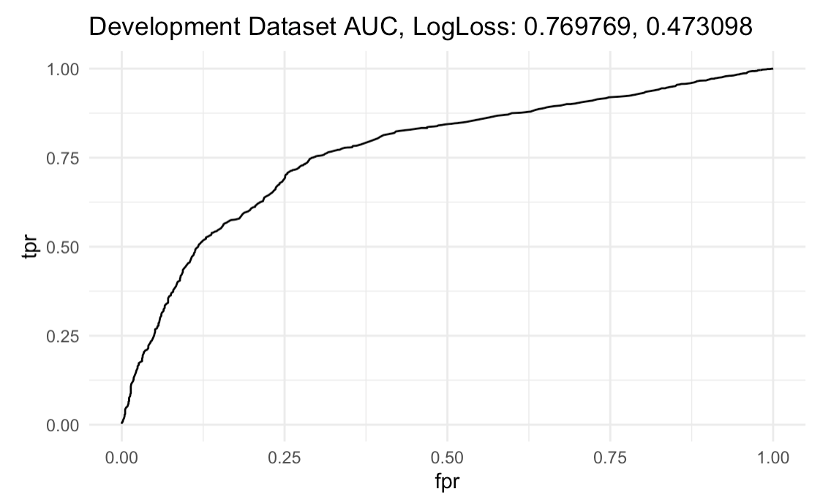
\includegraphics[width=15cm]{Q51.png} 
\caption{The ROC curve and associated AUC and log loss for the naïve Bayes classifier (measured using the development set)}
\label{R} %用于文内引用的标签
\end{figure} 	
 	\subsection{Logistic Regression}
 	\paragraph{} We first evaluated a simple logistic regression on the treatment group, visit day, and overall PANSS score (for the reasons described in the previous subsection). Figure 11 depicts the resultant ROC curve, in which we specify the development AUC and log loss as 0.6149 and 0.5499, respectively. While this is unquestionably an improvement over the Naive Bayes test error, we tried to reduce it further by including all of the individual PANSS values in the model.

\begin{figure}[H] 
\centering %
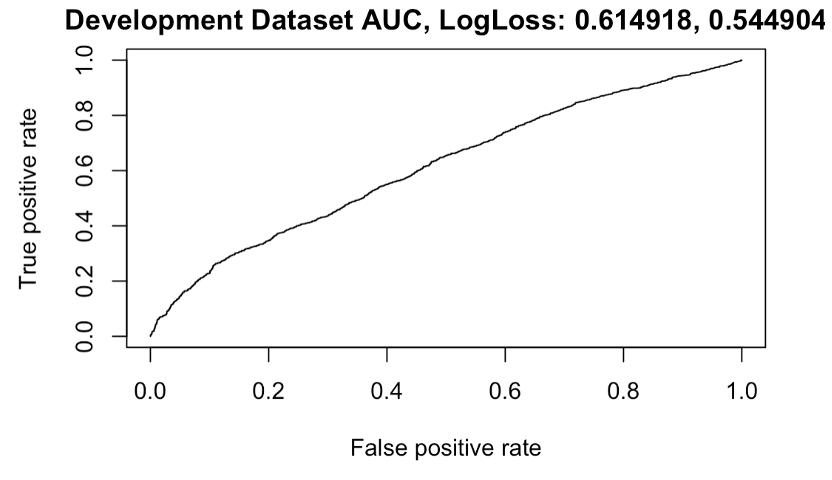
\includegraphics[width=15cm]{Q52.png} 
\caption{The ROC curve and associated AUC and log loss for logistic regression using only the total PANSS score (Development set) }
\label{R} %用于文内引用的标签
\end{figure} 
 \paragraph{}When evaluating each individual's PANSS score (and eliminating the entire PANSS score), we find an AUC and log loss of 0.6770 and 0.5224, respectively (Fig. 12). This indicates the possibility of overfitting since the apparent progress on the training set disappears when tested on the test set. Even though none of the development sets was utilized for training, our model has a small degree of bias because the training observations and development set observations only come from studies A to D. The test set only includes patients from study E. Consequently, our model contains a source of bias that we cannot directly address.
 
 	\paragraph{}The next move in our analysis was to consider the logistic regression model that considers all of the individual PANSS scores but to do feature selection by lasso to reduce the model variance (which should improve the test set score). In Figure 13, the ideal value of, the shrinkage value in lasso, is determined using cross-validation (10-folds). According to the one standard error criterion, the optimal value is so that only 24 predictors are evaluated. Therefore, we omit P1, P2, P6, G1, G6, G7, and G11 as predictors. Figure 14 shows the ROC curve for logistic regression with lasso and this specific value of = 0.00298 along with the AUC and log loss on the dev set. While log loss of 0.5238 is bigger than that observed in Fig. 12, the log loss for the test set is 0.5224, which is an improvement over the model that contains all of the individual PANSS scores. In this instance, the increase in bias caused by removing the abovementioned variables from our regression model resulted in a variance reduction sufficient to reduce the overall test error rate. This shows that limiting variation should be our priority if we intend to improve further our test set log loss.
 
 \begin{figure}[H] 
\centering %
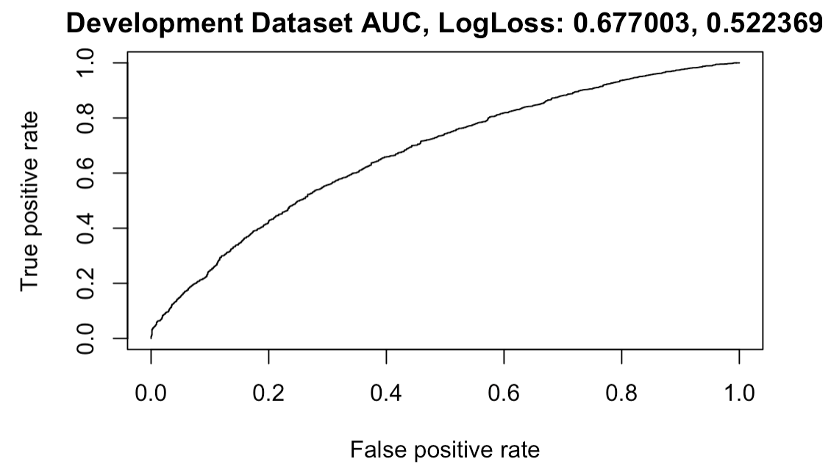
\includegraphics[width=15cm]{Q53.png} 
\caption{Determining the optimal shrinkage value for λ lasso in the context of our logistic regression on all individual PANSS scores.}
\label{R} %用于文内引用的标签
\end{figure} 

 \begin{figure}[H] 
\centering %
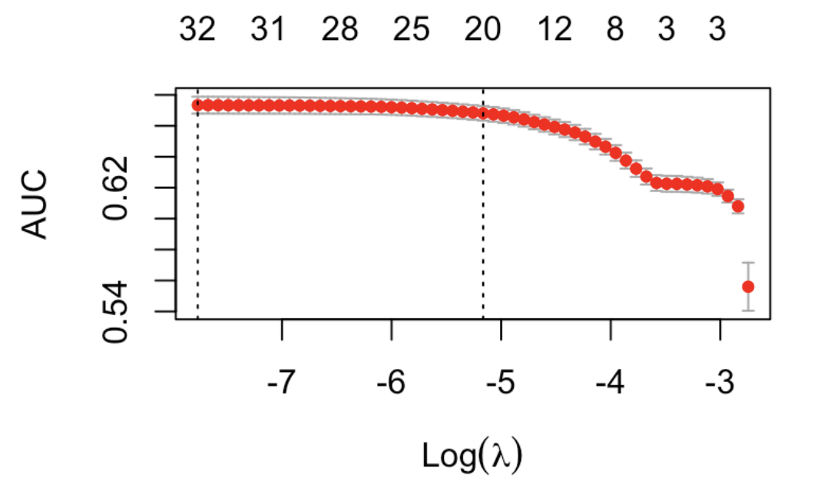
\includegraphics[width=15cm]{Q54.png} 
\caption{The ROC curve and associated AUC and log loss for logistic regression using all of the individual PANSS scores (Development set)}
\label{R} %用于文内引用的标签
\end{figure} 

 \begin{figure}[H] 
\centering %
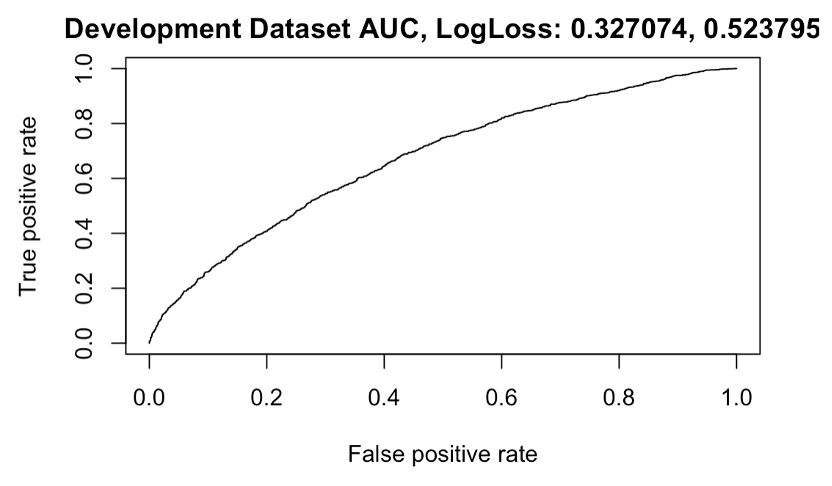
\includegraphics[width=15cm]{Q55.png} 
\caption{The ROC curve and associated AUC and log loss for logistic regression utilizing lasso (Development set)}
\label{R} %用于文内引用的标签
\end{figure} 


 	\subsection{Linear Discriminant Analysis}
 	\paragraph{}Next, we evaluated linear discriminant analysis as a classifier (LDA). Considering just treatment group, visit day, and PANSS total score as variables results in a model with slight variation (which, given the findings of the previous section, seems to be the best way to minimize our test error rate.) Not only is LDA effective for reducing our optimum test set error, but it may also assist us in comprehending the nature of the underlying data. This is accomplished by comparing the performance of LDA to that of other techniques and inferring the resulting influence on the dataset under the assumptions of multiple models. Figure 15 depicts the ROC curve for LDA, where the AUC and log loss on the design set are 0.6136 and 0.5454, respectively. LDA performs almost equally to our logistic regression using the complete PANSS score. Logistic regression and linear discriminant analysis (LDA) create a linear decision boundary; provided the underlying Bayes decision boundary is also linear, we anticipate both approaches to perform exceptionally well. Given that LDA assumes the observations in both classes are drawn from a Gaussian distribution, the equivalence in performance between the two approaches indicates that this is a reasonable assumption for this data set.
 	 \begin{figure}[H] 
\centering %
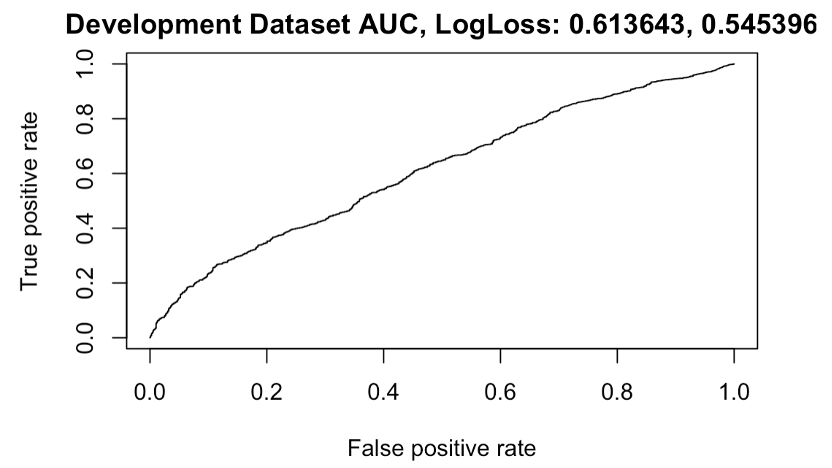
\includegraphics[width=15cm]{Q56.png} 
\caption{ The ROC curve and associated AUC and log loss for linear discriminant analysis (Development set)}
\label{R} %用于文内引用的标签
\end{figure} 
 	
 	
 	
 	\subsection{Quadratic Discriminant Analysis}
 	\paragraph{}Consideration is now given to quadratic discriminant analysis (QDA). If the decision boundary is somewhat nonlinear, we anticipate that QDA will perform better than LDA. Again, just the three predictions of treatment group, visit day, and PANSS total score are considered. The AUC and log loss for the dev set are shown in Figure 16 as 0.6568 and 0.5560, respectively. QDA does not perform poorly (relative to the majority of previously studied approaches) but is marginally inferior to LDA and our first logistic regression. Recall that QDA is distinct from LDA in that each class now has its covariance matrix - we no longer assume they are comparable. The decrease in bias, however, is accompanied by an increase in variance. This trade-off results in a net drop in our classifier's performance, which makes sense given that the best classifiers have been rigid.
 	
 	\begin{figure}[H] 
\centering %
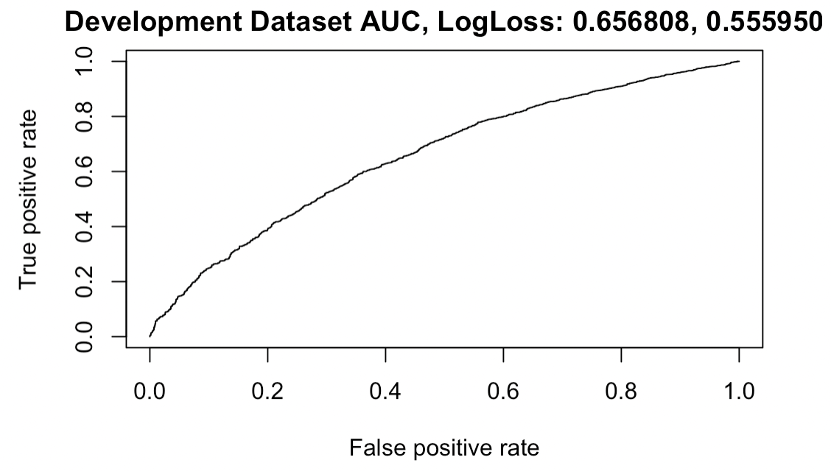
\includegraphics[width=15cm]{Q57.png} 
\caption{ The ROC curve and associated AUC and log loss for quadratic discriminant analysis (Development set)}
\label{R} %用于文内引用的标签
\end{figure} 
 	
% 	\subsection{Deep Neural Network}
% 	\paragraph{} Neural networks can be deemed as feature extractors and select important features to propagate forwards. All products of pairs of PANSS scores were added to features. Then, deep neural network with 0.2 dropout rate on input layer and 0.5 dropout rate on following hidden layers was trained. The dropout works in a manner similar to random forests, and prevents neural networks from overfitting the training set. To better corporate with dropout applied, activation functions for hidden layers were chosen to be ReLU, and the activation for the output layer was sigmoid.
% 	
% 	\paragraph{} After searching over hundreds of possible models, a deep neural network with five hidden layers and 1024 neurons on each hidden layer was selected. Moreover, a stop point at 150 epochs, training rate of 0.0003, and 512 batch size were used.
% 	
 	\subsection{The gradient boosting method and random forests}
 	\paragraph{}Gradient boosting method (GBM) and random forests were the final two models we investigated. Both approaches address the variance issue in the bias-variance tradeoff directly. Thus we anticipate that they will both function well with this dataset. GBM is accomplished by considering a collection of "weak" learners, often short trees (commonly stumps) that only permit fitting residuals at a slower pace. On the other hand, random forests reduce model variance by only examining a subset of the number of predictors per split in a given tree for a particular set of learners.
Figure 17 illustrates the effectiveness of the gradient boosting method (using XGBoost modified for random discrete grid search) when predictors including treatment group, visit day, and total PANSS score are used. Notably, the development set has an AUC of 0.7132 and a log-loss value of 0.5075. Our team noticed that we might not use the GBM's potential since it only utilizes three predictors. While previously introducing a single PANSS score decreased test set performance (due to greater model variance), we predict that GBM will not experience a similar setback because it concentrates on decreasing variance. Figure 18 depicts the ROC curves, related AUC, and log loss for GBM utilizing all PANSS values individually. The model obtained an AUC of 0.8194 and a log loss of 0.4201, indicating that the development set has increased significantly. However, this is not indicative of the test set's performance. By analyzing the relative significance of the different predictors in the modified GBM (Figure 19), we may acquire insight into the reasons behind this phenomenon. Note that the relative relevance, as determined by the $h2o.varimp_plot()$ function, largely takes into account the degree to which each predictor decreases the MSE at each step and the frequency with which a predictor is utilized to produce a split.
 \begin{figure}[H] 
\centering %
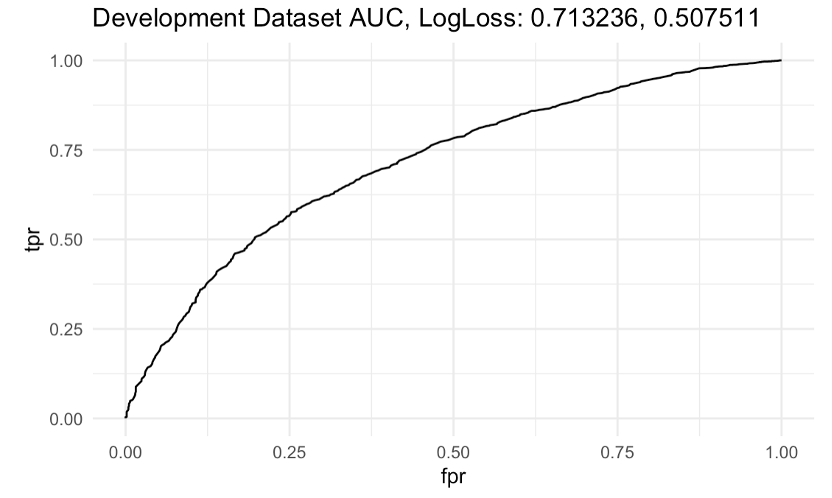
\includegraphics[width=15cm]{Q58.png} 
\caption{ The ROC curve and associated AUC and log loss for the gradient boosting method using the total PANSS score (Development set)}
\label{R} %用于文内引用的标签
\end{figure} 

\begin{figure}[H] 
\centering %
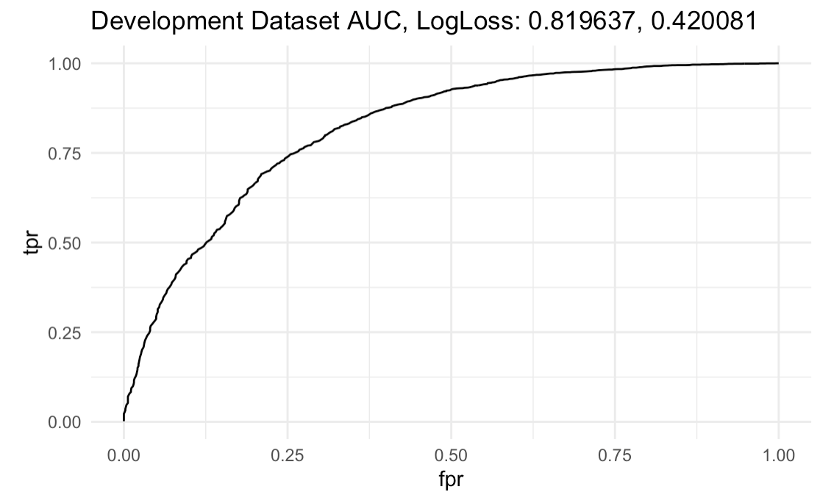
\includegraphics[width=15cm]{Q59.png} 
\caption{The ROC curve and associated AUC and log loss for the gradient boosting method using all individual PANSS scores (Development set)}
\label{R} %用于文内引用的标签
\end{figure}  

\begin{figure}[H] 
\centering %
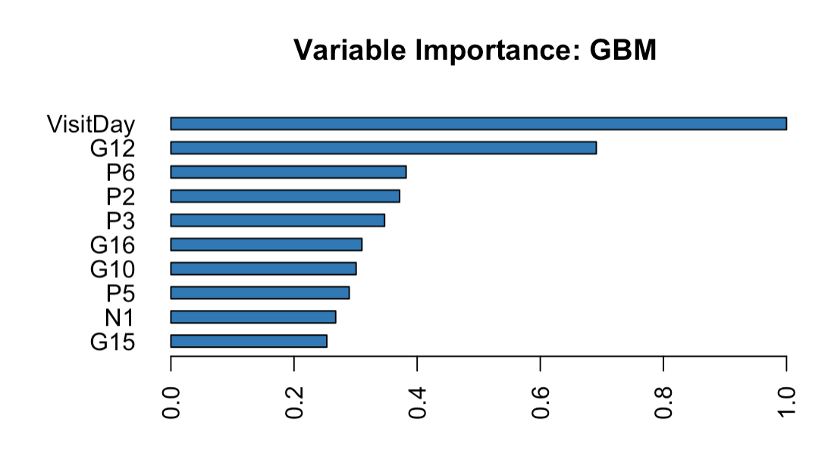
\includegraphics[width=15cm]{Q510.png} 
\caption{The relative variable importance for the gradient boosting method using all individuals PANSS score}
\label{R} %用于文内引用的标签
\end{figure}
\paragraph{}Predictors are used to determining the frequency of tree splits. The majority of PANSS scores fall within the positive and general symptom categories, as seen in the graph. In reality, just one of the first ten factors is linked to unfavorable symptoms (G15). Recalling Section 3, patients in Study E scored considerably differently than other patients on the first principal component, which was mostly associated with positive and general symptoms. This bias was again demonstrated on the test set as a decline in GBM performance.
\paragraph{}The random forest approach was the last method we investigated. On the development set, even a little overshooting time (again using random discrete grid search) is noteworthy (Figure 20). We observe the optimal AUC and log loss for the development set to be 0.8353 and 0.4108, respectively. We feel this pertains to the same issue as the gradient boosting approaches outlined before. For these methods to perform equally well on the test set, sophisticated methods for incorporating information from study E into the training set or manually adjusting the training set to more closely resemble the test set would need to be developed.

\begin{figure}[H] 
\centering %
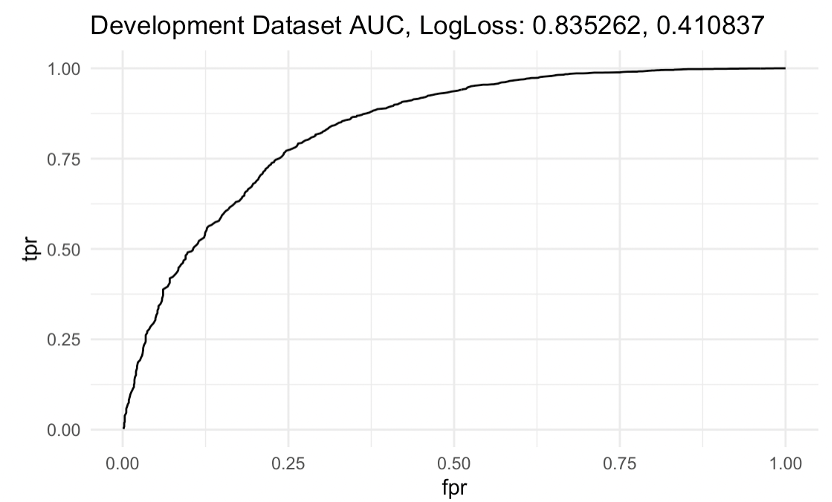
\includegraphics[width=15cm]{Q511.png} 
\caption{The ROC curve and associated AUC and log loss for the random forest method using all individual PANSS scores (Development set)}
\label{R} %用于文内引用的标签
\end{figure}

\subsection{Discussion}
 	\paragraph{}Generally, the least flexible approaches, such as logistic regression and LDA, fared the best. We ascribe this remarkable performance to the fact that patients in Study E scored considerably differently than patients in previous trials on the positive and general PANSS categories (as shown in Section 3). Since Study E patients were not included in the training set for the classification problem, we anticipated that the differences would provide a challenge for making predictions on the test set (i.e., all of Study E).
	\paragraph{}Attempting to tackle this issue using support vector machines (SVMs) might provide insight into why LDA and logistic regression seem superior to other approaches. In a preliminary examination of the use of SVMs in this dataset, we plotted observations from both categories on a plane spanned by visit day and PANSS total scores (Figure 21). This chart explains why the SVM did so badly overall (and why it is not covered in this report): it illustrates why the SVM fared so poorly. This graphic demonstrates that the data (at least when seen on this plane) are not segregated in any way. Therefore, we anticipate that the SVM will struggle to identify a correct hyperplane; all the "X" in the picture are support vectors (and the number of support vectors seems to be about the same as the total number of data points). In contrast, we discover that although logistic regression performs poorly with well-separated categories (i.e., its parameter values are unstable), it has no issues with continuous data. Even though the Bayesian error rate would be higher in this instance, logistic regression (and the closely related LDA) may still do well.

\begin{figure}[H] 
\centering %
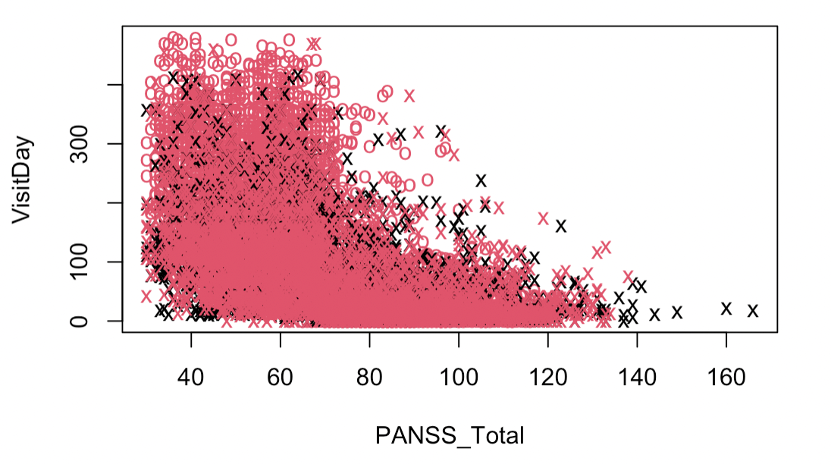
\includegraphics[width=15cm]{Q512.png} 
\caption{The ROC curve and associated AUC and log loss for the random forest method using all individual PANSS scores (Development set)}
\label{R} %用于文内引用的标签
\end{figure}

  \section{Appendix}
Kevin resposible for the "Patient segmentation" and analysis of that part;\\
Yunjie resposible for the "Treatment effect" and "Forecasting" and use latex to rewrite the report;\\
David resposible for the "Binary classification" and analysis of that part.\\




\end{document}